\chapter{Controls}
\label{ch:controls}
Control systems are responsible for computing the commands necessary for actuators to cause the trajectory of a system to go from its current state to a desired state. There are many different methods that can be used to determine the output commands. One of the more popular and widely implemented control systems is the PID (Proportional, Integral, Differential) controller. Lyapunov controllers utilize knowledge of the system dynamics to compute appropriate output commands. The robots in these experiments originally used PID controllers for position and heading control and were later tested with a Lyapunov contoller.

\section{PID}
\label{sec:pid}
PID controllers use the current state estimate to determine the errors between the desired state and the current state. The goal of the PID controller is to drive those errors to zero based on a number of criterion including rise time, settling time, steady state error and overshoot (see Figure \ref{fig:pid}).

\begin{figure}[ht!]
	\centering
	\includegraphics[width=.75\textwidth]{images/pid}
	\caption{PID controller output. The green line is the ideal output while the blue and purple lines are typical results. The orange line shows what happens when a system becomes unstable. Point $m$ represents the desired state, $m-n$ represents steady state error, point $a$ is the rise time and point $b$ is the settling time.}
	\label{fig:pid}
\end{figure}

There are separate PID controllers used for each of $x$ position, $y$ position and robot heading ($\psi$). The process used to compute an output using a PID controller uses three separate errors and a gain for each of those errors. Looking at the PID controller for heading the errors are

\begin{align}
\label{eq:piderrors}
\begin{split}
E_P &= \psi_{\text{ref}_k} - \psi_k \\
E_I &= \sum_{i=0}^{k}E_{P_i}*\Delta T \\
E_D &= \left(\psi_k - \psi_{k-1}\right)*\Delta T
\end{split}
\end{align}
where $\psi_{\text{ref}_k}$ is the desired heading at the current time, $\psi_k$ is the current heading estimate, $\psi_{k-1}$ is the previous heading estimate and $\Delta T$ is the time elapsed since the last PID control calculation was performed. The contribution of each error is then weighted by a gain to obtain the final output command, $u$, such that

\begin{align}
\label{eq:pidcommand}
u = K_P*E_P + K_I*E_I + K_D*E_D
\end{align}
where $K_P$ is the proportional gain, $K_I$ is the integral gain and $K_D$ is the differential gain.

The only parameters available to tune PID controllers for performance are the gains. There are some rules of thumb for tuning gains properly as described in \cite{ZeiglerNichols42} that can work as a good starting point. The difficulty in using PID controllers for the small robots used in these experiments is that the gains must be tuned for specific operating scenarios so that a set of gains that work well at full speed on asphalt do not work at all when the robot is driving in soft sand at any velocity. PID controllers work best when they only have to reject a small range of disturbances and the small robots are required to be operated in environments with a large range of disturbances.

When the characteristics of a robot are changed the PID gains must also be modified to reflect those changes. These characteristics include mass, center of mass, particular treads or motors and payloads, as these all affect the dynamics of the system. Gain scheduling is the process of tuning a system to use a different set of gains based on the operating environment or characteristics of the robot, however this is very time consuming. This motivates the search for a better control system for these small robots.

\section{Lyapunov}
\label{sec:lyapunov}
*** Talk about how Lyapunov controllers work \cite{Khalil02}. Show which control Lyapunov function I chose \cite{Rusu05RobotuxLyapunov}. For a given path show the linear and angular velocities that are output by each controller. ***